\section{Leitungen}

\subsection{Leitungsparameter}

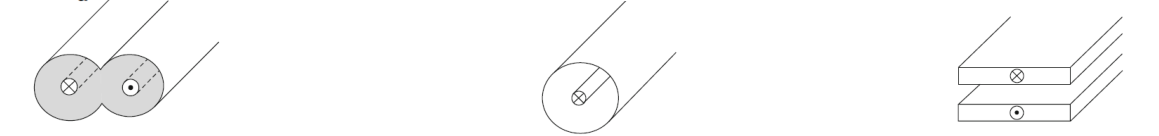
\includegraphics[width=\columnwidth]{Figures/Leitungsparameter.png}

\subsubsection{Doppelleitung:}
\begin{align*}
    a & = \text{Leiter Radius}                   & d & = \text{Abstand zw. den Leitern}                \\
    R & = \frac{1}{\pi a\delta\sigma_c}          & L & = \frac{\mu}{\pi} \cosh^{-1}\frac{d}{2a}      & \\
    G & = \frac{\pi\sigma}{\cosh^{-1}(^d/_{2a})} & C & = \frac{\pi\varepsilon}{\cosh^{-1}(^d/_{2a})}
\end{align*}

\subsubsection{Koaxial Leitung}
\begin{align*}
    a & = \text{innen Radius}                                              & b & = \text{äußerer Radius}               \\
    R & = \frac{1}{2\pi\delta\sigma_c}\left[\frac{1}{a}+\frac{1}{b}\right] & L & = \frac{\mu}{2\pi} \ln\frac{b}{a}     \\
    G & = \frac{2\pi\sigma}{\ln (^b/_a)}                                   & C & = \frac{2\pi\varepsilon}{\ln (^b/_a)}
\end{align*}

\subsubsection{Parallele Platten}
\begin{align*}
    w & = \text{Platten Breite}   & d & = \text{Abstand zw. Platten} \\
    R & = \frac{2}{w\delta\sigma} & L & = \frac{\mu d}{w}            \\
    G & = \frac{\sigma w}{d}      & C & = \frac{w\varepsilon}{d}
\end{align*}

Für beliebige Leitergeometrie gelten folgende Zusammenhänge:
\[
    LC = \mu\varepsilon \quad \text{und} \quad \frac{G}{C} = \frac{\sigma}{\varepsilon}
\]

\subsection{Übertragungsleitung mit Last}

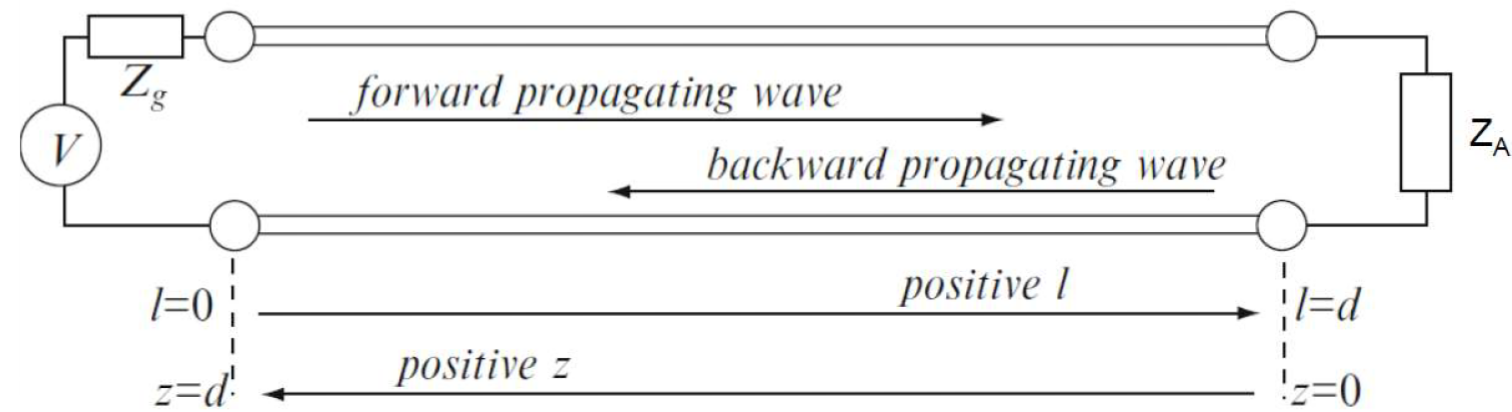
\includegraphics[width=\columnwidth]{Figures/UebertragungleitungmitLast.png}

\begin{align*}
    U(z) & = U^+ e^{\gamma z} + U^- e^{-\gamma z} = U^+ e^{\gamma d} + U^ - e^{-\gamma d}                      \\
    I(z) & = I^+ e^{\gamma z} + I^- e^{-\gamma z} = \frac{U^+}{Z_L}e^{\gamma d} - \frac{U^-}{Z_L}e^{-\gamma d}
\end{align*}

\begin{align*}
    \underline{z}_n & = \frac{\underline{Z}_A}{Z_L}                     & \underline{r} & = \frac{\underline{z}_n-1}{\underline{z}_n+1}= \frac{1-\underline{y}_n}{1+\underline{y}_n} \\
    \underline{r}_A & = \frac{\underline{Z}_A-Z_L}{\underline{Z}_A+Z_L} & m             & = \frac{1-|\underline{r}|}{1+|\underline{r}|}
\end{align*}
\subsubsection{Reflexionsfaktor entlang einer Leitung}

\begin{align*}
    r_E    & = r_A  ^{-2\gamma l} = r_A  e^{-2\alpha l} e^{-j2\beta l} \\
    \alpha & = -\frac{\ln(r_A)}{2l} [\si{Np/m}] & \beta  & = \dfrac{\phi_2 -\phi_1}{2l} [\si{rad/m}]
\end{align*}

\subsubsection{Stehwellenverhältnis}
\begin{align*}
    \mathrm{SWR} = \frac{U_\text{max}}{U_\text{min}} =
    \frac{I_\text{max}}{I_\text{min}} = \frac{1+|r(z)|}{1-|r(z)|} =
    \frac{|U_H|+|U_R|}{|U_H|-|U_R|}
\end{align*}
